\chapter{The ubiquitous equations chapter}
\index{quadratic}\index{equations!quadratic}
\section{Quadratic equations}
A quadratic equation takes the standard form
\begin{equation}
    a x^2 + b x + c = 0
\end{equation}\label{eqn:quadratic}
where \( a \), \( b \), and \( c \in \mathbb{Z} \) and \( a -neq 0 \). %
\index{quadratic!solutions}\index{equations!quadratic!solutions}%
A quadratic equation in its standard form has two solutions.
\begin{equation}
    x_{1,2} = - \frac{b \pm \sqrt{b^2 - 4 a c}}{2a}
\end{equation}\label{eqn:quadsolns}
\index{determinant}\index{quadratic!determinant}\index{equations!quadratic!determinant}%
If the determinant of a quadratic equation,
\begin{equation}
    \Delta = b^2 - 4 a c
\end{equation}
is zero, then the solutions coalesce to a single value \( x \in \mathbb{Q} \):
\begin{equation}
    x = - \frac{b}{2a}
\end{equation}
The plot of a sample quadratic function, \( y = x^2 - 2 \), can be seen in \Cref{fig:quadplot}.

\index{quadratic!plot}\index{equations!quadratic!plot}
\begin{figure}[htbp!]
    \centering
    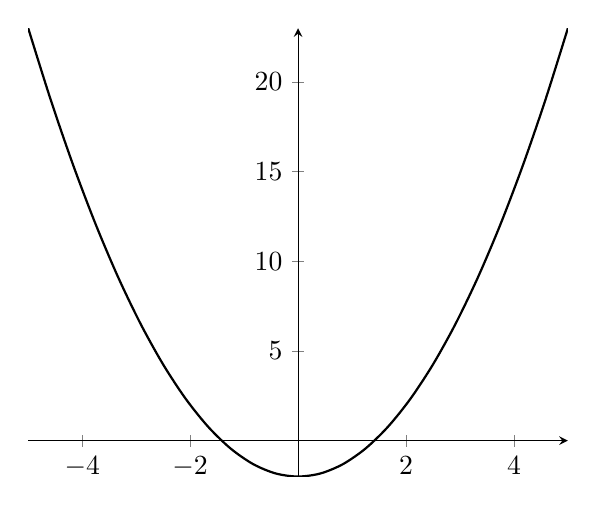
\begin{tikzpicture}
        \begin{axis}[axis lines=center]
            \addplot[domain=-5:5, thick, smooth]{x^2-2};
        \end{axis}
    \end{tikzpicture}
    \caption{Plot of the equation \( y = x^2 - 2 \).}
    \label{fig:quadplot}
\end{figure}

\index{saddle point}
\section{\Gls{saddlepoint}}
A \gls{saddlepoint} (a.k.a. \gls{minimax}) is a point on a three-dimensional surface where
tangental slopes (i.e., derivatives) in the orthogonal directions are zero, but the point
itself is not a local extremum. A classic example, \( f(x, y) = x^2 - y^2 \), is depicted in
\Cref{fig:saddle}.

\index{saddle point!plot}
\begin{figure}[htbp!]
    \centering
    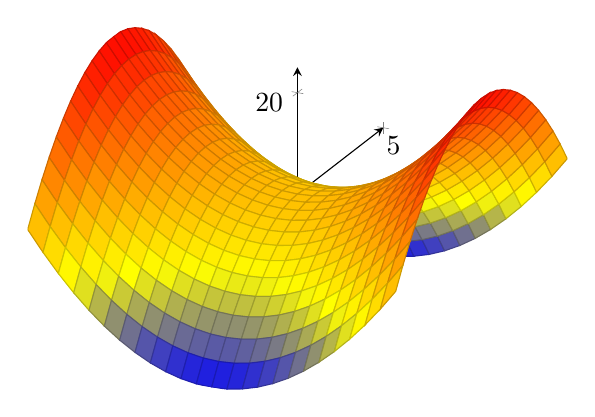
\begin{tikzpicture}
        \begin{axis}[axis lines=center]
            \addplot3[surf,domain=-5:5]{x^2-y^2};
        \end{axis}
    \end{tikzpicture}
    \caption{Plot of the equation \( z = x^2 - y^2 \).}
    \label{fig:saddle}
\end{figure}

\section{More mathematics examples}
These examples are taken from \autocite{fre2021}.

\LaTeX\ is a great program for writing math. I can write inline
math such as \( a^2 + b^2 = c^2 \). I also can give equations
their own space:

\begin{equation}
    \gamma^2 + \theta^2 = \omega^2
\end{equation}

\subsection{Maxwell's equations}
\index{equations!Maxwell's}\index{Maxwell's equations}
Maxwell's equations are named for James Clark Maxwell and are as follows:
\nopagebreak
\begin{align}
    \vec{\nabla} \cdot \vec{E} \quad  & = \quad \frac{\rho}{\epsilon_0} & \text{Gauss's law} \\
    \vec{\nabla} \cdot \vec{B} \quad  & = \quad 0 & \text{Gauss's law for magnetism} \\
    \vec{\nabla} \times \vec{E} \quad & = \quad - \frac{\partial\vec{B}}{\partial t} & \text{Faraday's law of induction} \\
    \vec{\nabla} \times \vec{B} \quad & = \quad \mu_0 \left(\epsilon_0\frac{\partial\vec{E}}{\partial t} + \vec{J}\right) & \text{Ampere's circuital law}
\end{align}

\subsection{Matrix equations}
\begin{equation}
    \begin{pmatrix}
        a_{11} & a_{12} & \cdots & a_{1n} \\
        a_{21} & a_{22} & \cdots & a_{2n} \\
        \vdots & \vdots & \ddots & \vdots \\
        a_{n1} & a_{n2} & \cdots & a_{nn}
    \end{pmatrix}            
    \begin{bmatrix}
        v_1 \\
        v_2 \\
        \vdots \\
        v_n
    \end{bmatrix}
    =
    \begin{matrix}
        w_1 \\
        w_2 \\
        \vdots \\
        w_n
    \end{matrix}
\end{equation}

\subsection{Some additional equations}
\begin{equation}
    \int_a^b x \, dx = \left.\frac{x^2}{2} \right|_a^b
\end{equation}

\begin{equation}
    \iiint\limits_V f(x,y,z) \, dV = F
\end{equation}

\begin{equation}
    \frac{dx}{dy} = x' = \lim_{h \to 0} \frac{f(x + h) - f(x)}{h}
\end{equation}

\begin{equation}
    \left| x \right| =
    \begin{cases}
        -x, & \text{if} \, x < 0 \\
        x,  & \text{if} \, x \geq 0
    \end{cases}
\end{equation}

\begin{equation}
    F(x) = A_0 + \sum_{n=1}^N \left[ A_n \cos \left( \frac{2 \pi n x}{P} \right) + B_n \sin \left( \frac{2 \pi n x}{P} \right) \right]
\end{equation}

\begin{equation}
    \sum_n \frac{1}{n^s} = \prod_p \frac{1}{1 - \frac{1}{p^s}}
\end{equation}

\begin{equation}
    m \ddot{x} + c \dot{x} + k x = F_0 \sin \left( 2 \pi f t \right)
\end{equation}

\begin{align}
    f(x) \quad & = \quad x^2 + 3x + 5x^2 + 8 + 6x \\
         \quad & = \quad 6x^2 + 9x + 8 \\
         \quad & = \quad x(6 x + 9) + 8
\end{align}

\begin{equation}
    X = \frac{F_0}{k} \frac{1}{\sqrt{(1 - r^2)^2 + (2 \zeta r)^2}}
\end{equation}

\begin{equation}
    G_{\mu\nu} \equiv R_{\mu\nu} - \frac{1}{2} R g_{\mu\nu} = \frac{8 \pi G}{c^4} T_{\mu\nu}
\end{equation}

\begin{equation}
    \ch{6 CO2 + 6 H2O -> C6H12O6 + 6 O2} % Fails with babel and certain languages
\end{equation}

\begin{equation}
    \ch{SO4^2- + Ba^2+ -> BaSO4} % Fails with babel and certain languages
\end{equation}

\begin{equation}
    \frac{\partial{\bf{u}}}{\partial{t}}+(\bf{u}\cdot\nabla)\bf{u}-\nu\nabla^2\bf(u)=-\nabla h
\end{equation}